\section{Date: 2026-09-11}
\noindent \textbf{Series ID: A034RC1A027NBEA} 

\noindent This series is titled National income: Compensation of employees: Wages and salaries and has a frequency of Annual. The units are Billions of Dollars and the seasonal adjustment is Not Seasonally Adjusted.The observation start date is 1929-01-01 and the observation end date is 2025-01-01.The popularity of this series is 23. \\ 

\noindent \textbf{Series ID: OGDE249MFGN} 

\noindent This series is titled All Employees: Manufacturing in Ogden, UT (MSA) and has a frequency of Monthly. The units are Thousands of Persons and the seasonal adjustment is Not Seasonally Adjusted.The observation start date is 1990-01-01 and the observation end date is 2026-07-01.The popularity of this series is 1. \\ 

\subsection{Raw Regression}
\noindent Regresses the two series against each other directly. A significant result here can come just as easily from both series sharing a long-run trend as from any real relationship.

\begin{center}
\begin{tabular}{lclc}
\toprule
\textbf{Dep. Variable:}               & value\_fred\_OGDE249MFGN & \textbf{  R-squared:         } &     0.802   \\
\textbf{Model:}                       &           OLS            & \textbf{  Adj. R-squared:    } &     0.797   \\
\textbf{Method:}                      &      Least Squares       & \textbf{  F-statistic:       } &     138.0   \\
\textbf{Date:}                        &     Fri, 11 Sep 2026     & \textbf{  Prob (F-statistic):} &  1.62e-13   \\
\textbf{Time:}                        &         15:19:38         & \textbf{  Log-Likelihood:    } &   -76.434   \\
\textbf{No. Observations:}            &              36          & \textbf{  AIC:               } &     156.9   \\
\textbf{Df Residuals:}                &              34          & \textbf{  BIC:               } &     160.0   \\
\textbf{Df Model:}                    &               1          & \textbf{                     } &             \\
\textbf{Covariance Type:}             &        nonrobust         & \textbf{                     } &             \\
\bottomrule
\end{tabular}
\begin{tabular}{lcccccc}
                                      & \textbf{coef} & \textbf{std err} & \textbf{t} & \textbf{P$> |$t$|$} & \textbf{[0.025} & \textbf{0.975]}  \\
\midrule
\textbf{const}                        &      14.0195  &        0.885     &    15.840  &         0.000        &       12.221    &       15.818     \\
\textbf{value\_fred\_A034RC1A027NBEA} &       0.0015  &        0.000     &    11.748  &         0.000        &        0.001    &        0.002     \\
\bottomrule
\end{tabular}
\begin{tabular}{lclc}
\textbf{Omnibus:}       &  2.395 & \textbf{  Durbin-Watson:     } &    0.177  \\
\textbf{Prob(Omnibus):} &  0.302 & \textbf{  Jarque-Bera (JB):  } &    1.478  \\
\textbf{Skew:}          &  0.221 & \textbf{  Prob(JB):          } &    0.478  \\
\textbf{Kurtosis:}      &  2.111 & \textbf{  Cond. No.          } & 1.82e+04  \\
\bottomrule
\end{tabular}
%\caption{OLS Regression Results}
\end{center}

Notes: \newline
 [1] Standard Errors assume that the covariance matrix of the errors is correctly specified. \newline
 [2] The condition number is large, 1.82e+04. This might indicate that there are \newline
 strong multicollinearity or other numerical problems.

\begin{figure}
\centering
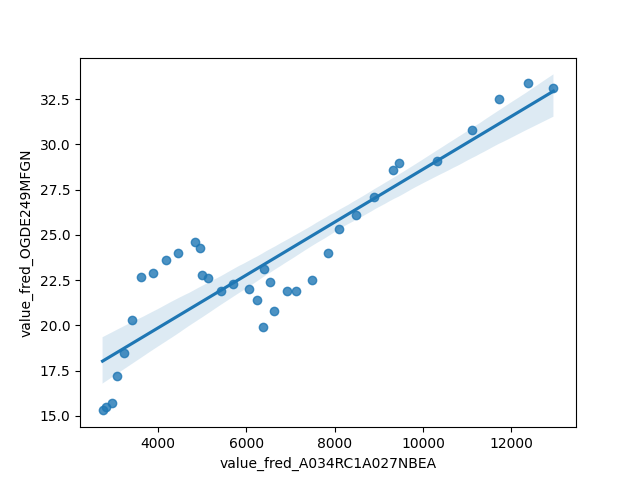
\includegraphics[scale = 0.9]{plots/plot_2026-09-11.png}
\caption{Raw Regression Plot for 2026-09-11}
\end{figure}
\newpage
\subsection{Detrended Regression}
\noindent Regresses the residuals of each series after removing its own linear time trend, so a shared trend can no longer drive the result on its own. A relationship that stays significant here is better evidence of a genuine link between the two series.

\begin{center}
\begin{tabular}{lclc}
\toprule
\textbf{Dep. Variable:}                          & value\_fred\_OGDE249MFGN\_detrended & \textbf{  R-squared:         } &     0.401   \\
\textbf{Model:}                                  &                 OLS                 & \textbf{  Adj. R-squared:    } &     0.383   \\
\textbf{Method:}                                 &            Least Squares            & \textbf{  F-statistic:       } &     22.75   \\
\textbf{Date:}                                   &           Fri, 11 Sep 2026          & \textbf{  Prob (F-statistic):} &  3.40e-05   \\
\textbf{Time:}                                   &               15:19:38              & \textbf{  Log-Likelihood:    } &   -74.459   \\
\textbf{No. Observations:}                       &                    36               & \textbf{  AIC:               } &     152.9   \\
\textbf{Df Residuals:}                           &                    34               & \textbf{  BIC:               } &     156.1   \\
\textbf{Df Model:}                               &                     1               & \textbf{                     } &             \\
\textbf{Covariance Type:}                        &              nonrobust              & \textbf{                     } &             \\
\bottomrule
\end{tabular}
\begin{tabular}{lcccccc}
                                                 & \textbf{coef} & \textbf{std err} & \textbf{t} & \textbf{P$> |$t$|$} & \textbf{[0.025} & \textbf{0.975]}  \\
\midrule
\textbf{const}                                   &   -5.583e-14  &        0.328     &  -1.7e-13  &         1.000        &       -0.667    &        0.667     \\
\textbf{value\_fred\_A034RC1A027NBEA\_detrended} &       0.0025  &        0.001     &     4.770  &         0.000        &        0.001    &        0.004     \\
\bottomrule
\end{tabular}
\begin{tabular}{lclc}
\textbf{Omnibus:}       &  0.572 & \textbf{  Durbin-Watson:     } &    0.205  \\
\textbf{Prob(Omnibus):} &  0.751 & \textbf{  Jarque-Bera (JB):  } &    0.649  \\
\textbf{Skew:}          &  0.067 & \textbf{  Prob(JB):          } &    0.723  \\
\textbf{Kurtosis:}      &  2.356 & \textbf{  Cond. No.          } &     638.  \\
\bottomrule
\end{tabular}
%\caption{OLS Regression Results}
\end{center}

Notes: \newline
 [1] Standard Errors assume that the covariance matrix of the errors is correctly specified.

\begin{figure}
\centering
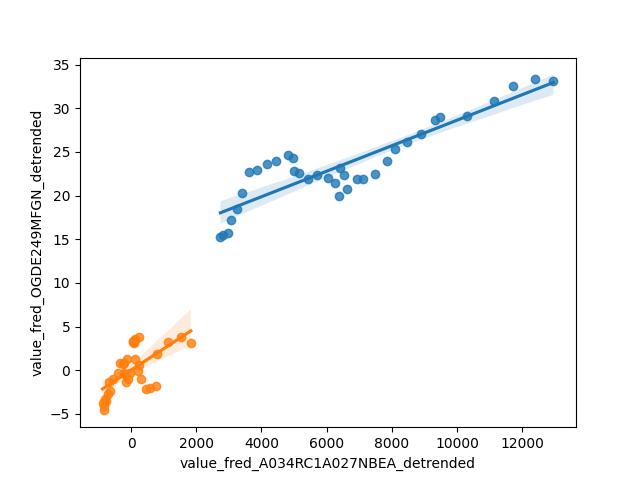
\includegraphics[scale = 0.9]{plots/plot_2026-09-11_detrended.png}
\caption{Detrended Regression Plot for 2026-09-11}
\end{figure}
\newpage
